\section{Parameterization Methods}


\subsection{CGAL::parameterize()}

From the user's point of view, this package provides a second entry point
where the user may specify a parameterization method (including a border
parameterization method and a linear solver):

\ccFunction{Parametizer_traits_3<MeshAdaptor_3>::Error_code parameterize (MeshAdaptor_3 * mesh, ParametizerTraits_3 parametizer);}
{
Compute a 1 to 1 mapping from a triangular 3D surface 'mesh' to a piece of the 2D space. The mapping is linear by pieces (linear in each triangle). The result is the (u,v) pair image of each vertex of the 3D surface.
1 to 1 mapping may be guaranteed or not, depending of ParametizerTraits\_3 algorithm chosen.
Preconditions:\begin{itemize}
\item 'mesh' must be a surface with 1 connected component.\item 'mesh' must be a triangular mesh.\item the mesh border must be mapped onto a convex polygon (for fixed border parameterizations).\end{itemize}
}
\begin{description}
\item[Parameters: ]
\begin{description}
\item[mesh]3D mesh, model of MeshAdaptor\_3 \item[parametizer]Parameterization method for 'mesh' \end{description}
\end{description}


\subsection{Parameterization Methods List}

This \cgal\ package implements some of the state-of-the-art
parameterization methods as models of the ParametizerTraits\_3 concept:

\begin{itemize}

\item Fixed boundary:

    \begin{itemize}

    \item Tutte uniform weights (guaranteed one-to-one mapping for
    convex boundary)

    \ccRefIdfierPage{CGAL::Barycentric_mapping_parametizer_3}  \\

    \item Mean coordinate values (ditto)

    \ccRefIdfierPage{CGAL::Mean_value_coordinates_parametizer_3}  \\

    \item Discrete conformal maps (conditionally guaranteed if all
    weights positive and convex boundary)

    \ccRefIdfierPage{CGAL::Discrete_conformal_map_parametizer_3}  \\

    \item Authalic (ditto)

    \ccRefIdfierPage{CGAL::Discrete_authalic_parametizer_3}  \\

    \end{itemize}

\item Free boundary:

    \begin{itemize}

    \item Least squares conformal maps

    \ccRefIdfierPage{CGAL::LSCM_parametizer_3}  \\

    \item Discrete conformal maps

    (not yet implemented)

    \end{itemize}

\end{itemize}


\subsection{Authalic Parameterization Example}

The code below applies a Discrete Authalic parameterization to a Polyhedron\_3 mesh:

\begin{ccExampleCode}

// CGAL kernel
typedef CGAL::Cartesian<double>                         Kernel;

// Mesh true type and parameterization adaptors
typedef CGAL::Polyhedron_3<Kernel>                      Polyhedron;
typedef CGAL::Mesh_adaptor_polyhedron_3<Polyhedron>     Mesh_adaptor_polyhedron;

// Discrete Authalic parametizer
typedef CGAL::Discrete_authalic_parametizer_3<Mesh_adaptor_polyhedron>
                                                        Parametizer;

int main(int argc,char * argv[])
{
    Polyhedron mesh;
    ...

    // The parameterization package needs an adaptor to handle Polyhedron_3 meshes
    // Note: parameterization methods support only meshes that are toplogical disks
    Mesh_adaptor_polyhedron mesh_adaptor(&mesh);

    // Discrete Authalic parameterization
    Parametizer::Error_code err = CGAL::parameterize(&mesh_adaptor, Parametizer());
    ...
}

\end{ccExampleCode}

See the complete code in Polyhedron\_parameterization2.C example.

% Include authalic.png/eps figure with title = "Discrete Authalic parameterization"
\begin{figure}[bht]
    \begin{center}
        % Image
        \begin{ccTexOnly}
            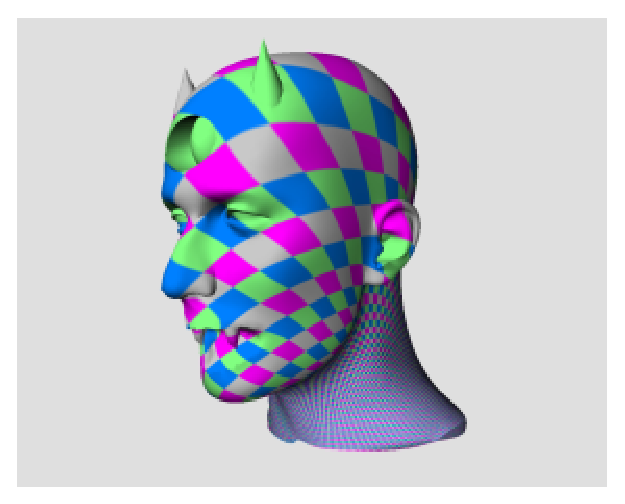
\includegraphics{Parameterization/authalic} % omit suffix to support PS and PDF
        \end{ccTexOnly}
        \begin{ccHtmlOnly}
            <img border=0 src="./authalic.png" align=center>
        \end{ccHtmlOnly}
        \label{parameterization-fig-authalic}

        % Title
        \caption{Discrete Authalic parameterization}
    \end{center}
\end{figure}


\subsection{Boundary parameterization Methods List}

Boundary parameterization methods define a
set of constraints (a constraint specifies two u,v coordinates for
each instance of a vertex along the boundary).

This package implements classic boundary parameterization methods
as models of the BorderParametizer\_3 concept. They are used as traits classes
modifying the behavior of the parameterization methods above.

\begin{itemize}

\item For free boundary methods: only two constraints (the pinned
vertices). They have to be on the specified boundary.

\ccRefIdfierPage{CGAL::Two_vertices_parametizer_3}  \\

\item For fixed boundary methods:

    \begin{itemize}

    \item the user can select a boundary
        parameterization among two common methods: uniform or
        arc-length parameterization.

    \item one convex shape specified by:

        \begin{itemize}

        \item one shape among a set of standard ones (circle, square).

        \item a convex polygon.

        \end{itemize}

    \end{itemize}

    \ccRefIdfierPage{CGAL::Circular_border_arc_length_parametizer_3}  \\
    \ccRefIdfierPage{CGAL::Circular_border_uniform_parametizer_3}  \\
    \ccRefIdfierPage{CGAL::Square_border_arc_length_parametizer_3}  \\
    \ccRefIdfierPage{CGAL::Square_border_uniform_parametizer_3}  \\

\end{itemize}


\subsection{Square Border Arc Length Parameterization Example}

The code below applies a Floater's mean value coordinates parameterization
with a Square Border Arc Length Parameterization:

\begin{ccExampleCode}

// CGAL kernel
typedef CGAL::Cartesian<double>                         Kernel;

// Mesh true type and parameterization adaptors
typedef CGAL::Polyhedron_3<Kernel>                      Polyhedron;
typedef CGAL::Mesh_adaptor_polyhedron_3<Polyhedron>     Mesh_adaptor_polyhedron;

// Square border parametizer
typedef CGAL::Square_border_arc_length_parametizer_3<Mesh_adaptor_polyhedron>
                                                      Border_parametizer;

// Floater's mean value coordinates parametizer with square border
typedef CGAL::Mean_value_coordinates_parametizer_3<Mesh_adaptor_polyhedron,
                                                    Border_parametizer>
                                                        Parametizer;

int main(int argc,char * argv[])
{
    Polyhedron mesh;
    ...

    // The parameterization package needs an adaptor to handle Polyhedron_3 meshes
    // Note: parameterization methods support only meshes that are toplogical disks
    Mesh_adaptor_polyhedron mesh_adaptor(&mesh);

    // Floater's mean value coordinates parameterization
    // with a Square Border Arc Length Parameterization
    Parametizer::Error_code err = CGAL::parameterize(&mesh_adaptor, Parametizer());
    ...
}

\end{ccExampleCode}

See the complete code in Polyhedron\_parameterization3.C example.
